To evaluate our autoscaling system described above, we ran experiments
on two infrastructures: a homogeneous one (the DAS-4, a multi-cluster system
hosted by universities in The Netherlands~\cite{das4}) and a heterogeneous
one (the Amazon EC2 cloud~\cite{amazonEC2}). The goal of our experiments
was to evaluate and compare different scaling plans by how well they react under sudden
workload changes (e.g. a network outage). In particular, our evaluation focus on
the SLO fulfillment, amount and type of resources the scaling plans allocated to handle
this traffic anomaly. 

%In this section we conducted our experiments on a heterogeneous infrastructure like Amazon EC2~\cite{amazonEC2}, and on a homogeneous infrastructure like DAS-4 (the Distributed ASCI Supercomputer 4)~\cite{das4}. In our experiment campaign, we compared the degree of SLO enforcement and resource consumption for each provisioning algorithm implemented in ConPaaS. 

%DAS-4 is the Dutch Computational Infrastructure, a six-cluster wide-area distributed system designed with research purposes

\textbf{Testbed configuration:}  As a representative scenario, we deployed the MediaWiki~\cite{mediawiki} application using ConPaaS~\cite{conpaasIC} on both infrastructures. ConPaaS is an open-source runtime environment for hosting applications in Cloud infrastructures. To run the MediaWiki application, we used the WikiBench benchmark~\cite{wikibench}. This benchmark uses a full copy of Wikipedia as the web application, and replays a fraction of the actual Wikipedia's access traces. 

Given such a scenario, ConPaaS provides support for all the required services to host a copy of Wikipedia: a PHP web hosting and a MySQL service. The MySQL service is loaded with a full copy of the English Wikipedia articles as of 2011, which has a size of approximately 40GB.  In the PHP service, the configuration was composed of one load balancer, one or more static web server and one or more PHP servers. For these experiments, we focus on the elasticity of the PHP tier, and in particular how the number of vm's hosting PHP servers will grow and shrink on demand.

For monitoring-data analysis, ConPaaS provides a monitoring component based on Ganglia~\cite{ganglia}, a scalable distributed monitoring system. We implemented modules that extend Ganglia's standard set of monitoring metrics by adding a number of service-specific metric for measuring the request rate and response times of static and dynamic requests.

 

%The architecture of ConPaaS services comprises two main building blocks: agents and managers.  The agent VMs host the needed components to provide the service-specific functionality. While the manager is in charge of centralizing monitoring data, controlling the allocation of resources, and coordinating reconfigurations when adding or removing resources. 



% and we ran the Wikibench tools with a 10\% sample of a real Wikipedia access trace for 24hours. 
%Instead of basing our evaluations on unrealistic workloads,


%We then use WikiBench to replay access traces from 2011~\cite{urdaneta2009}.

%Consequently, our goal is to evaluate the behavior of the provisioning algorithms, when scaling out and back the number of VMs hosting PhP servers to guarantee several performance requirements, referred to as SLO.  Accordingly, some assumptions were made:
We configured the experiments as follows:


\begin{itemize}
%\item  Response times from static requests were not analyzed due to its lightweight nature. 

\item The monitoring data was collected over a reporting period of 5 minutes.

\item We fixed a SLO of 700 milliseconds at the service's side.

\item We fixed a SLO penalty per violation to half the price of a small instance in DAS-4 and EC2 infrastructures.

%\item The algorithms used the same statistically-chosen performance threshold ranges. 

\item A minimum interval of 10 minutes has been established between scaling actions to avoid excessive oscillations. 
\end{itemize}


%To provide the Wikipedia services, an initial configuration was composed of 4 VMs, and 1 VM to host the Wikibench tools. The 4 VMs include a PhP service manager VM, a PhP agent VM, a web server and a http-proxy agent VM (both in the same VM), and finally a MySQL agent VM to store the English Wikipedia data, as explained in Section~\ref{wikipedia}.


\textbf{Workload trace:}  Instead of using unrealistic and synthetic workloads generated by benchmark tools, such as TPC-W, RuBiS and RuBBoS, we ran the Wikibench tools with a 10\% sample of a real Wikipedia access trace from 2011.  This trace contains requests for static pages as well as dynamic PHP requests. As mentioned above, the most important performance bottleneck is the application logic of the application: PHP requests are processed an order of magnitude slower than simpler static web pages. Figure~\ref{workload} plots the PHP workload sampled from one trace, as the number of PHP requests per minute during approximately three days. One interesting aspect that we noticed about this trace is a sudden drop in the workload during a period of time of 17min. By looking at the traffic logs, it seems that the access traces were not written into the logs due to an anomaly probably caused by a network outage or power shutdown. 

\begin{figure}
\begin{center}
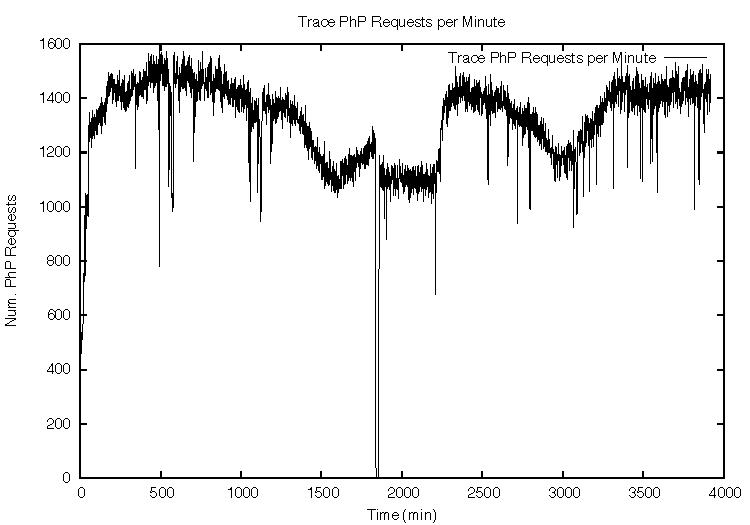
\includegraphics[width=0.49\textwidth, height=6cm]{./images/traceWorkload2011}
\end{center}
\vspace{-5mm}
\caption{Wikipedia trace workload.}
\label{workload}
\end{figure}

In this article we therefore focus on the automatic scaling of the PHP tier during this outage.

\subsection{Heterogeneous Infrastructure}

Initially, our experiments on EC2 used small instances for the PHP service and one large instance for the MySQL service. Table~\ref{EC2instances} details the available configurations of the different types of instances in EC2.

\begin{table}
  {\scriptsize 
\begin{center}
    \begin{tabular}{  | c | c | c | c | c |}
    \hline
      \textbf{Name}  & \textbf{Configuration} & \textbf{Cost/hr} \\ \hline
   \textit{m1.small}   & 1-ECU~\footnote{One EC2 compute unit provides the equivalent CPU capacity of a 1.0-1.2 GHz 2007 Opteron or 2007 Xeon processor.}  -- 1.5Gb RAM&  0.06\$ \\ \hline
   \textit{m1.medium}   & 2-ECU -- 4Gb RAM&  0.12\$ \\ \hline
\textit{c1.medium} & 5-ECU -- 3Gb RAM& 0.145\$   \\ \hline
\textit{m1.large} & 4-ECU -- 8Gb RAM& 0.24\$   \\ \hline
 \end{tabular}
\end{center}
\vspace{-5mm}
\caption{EC2 instance type characteristics.}
\label{EC2instances}
}
\end{table}

\paragraph{SLA fulfillment}

\begin{figure*}[htb]
	\begin{minipage}[b]{0.32\linewidth}
		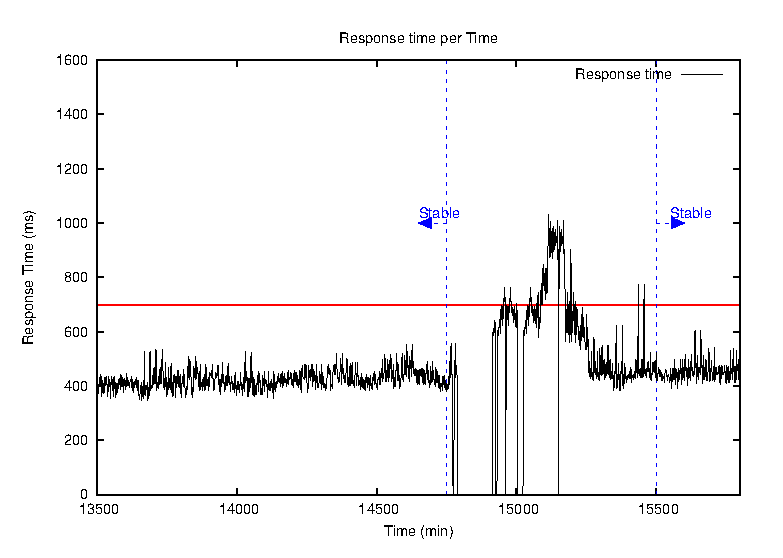
\includegraphics[height=4cm]{images/exps2011/low/ec2/proxyDataPoints_output_filtered.eps}	
		\vspace{-4mm}
	\end{minipage}
	\hfill
	\begin{minipage}[b]{0.32\linewidth}
		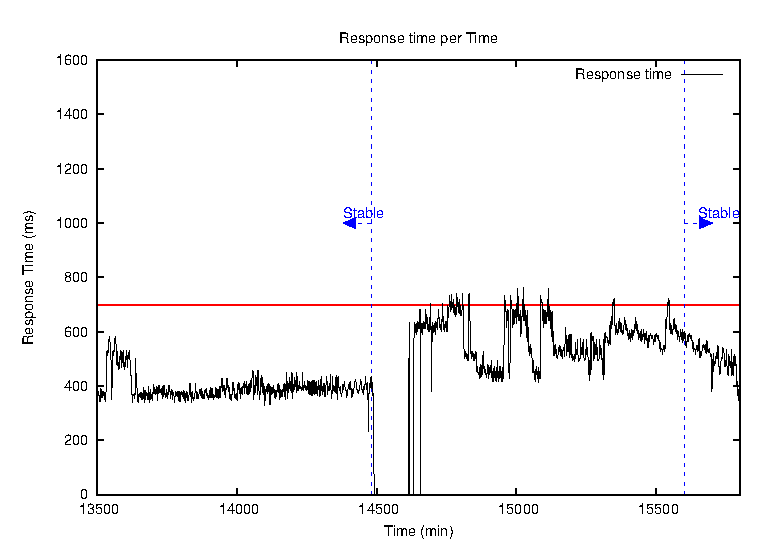
\includegraphics[height=4cm]{images/exps2011/medium/ec2/proxyDataPoints_output_filtered.eps}
		\vspace{-4mm}
	\end{minipage}
\hfill
\begin{minipage}[b]{0.32\linewidth}
		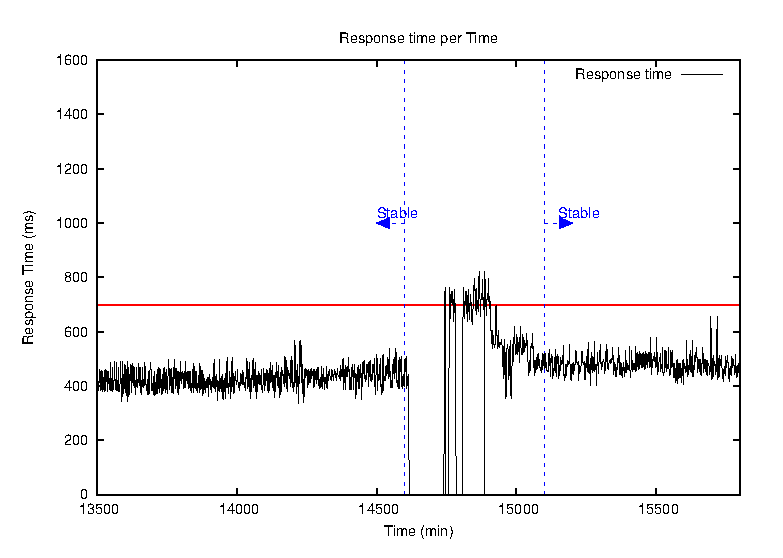
\includegraphics[height=4cm]{images/exps2011/high/ec2/proxyDataPoints_output_filtered.eps}
		\vspace{-4mm}
	\end{minipage}
\caption{Response time values during the outage.}
\label{fig:EC2ResponseTime}
\end{figure*}

\paragraph{Resource consumption}

\begin{figure*}[htb]
	\begin{minipage}[b]{0.32\linewidth}
		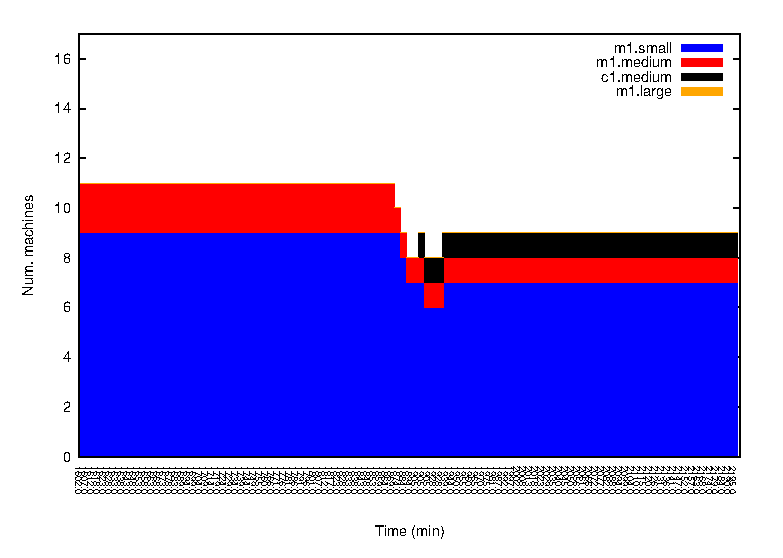
\includegraphics[height=4cm]{images/exps2011/low/ec2/inst_type_machines_filtered.eps}	
		\vspace{-4mm}
	\end{minipage}
	\hfill
	\begin{minipage}[b]{0.32\linewidth}
		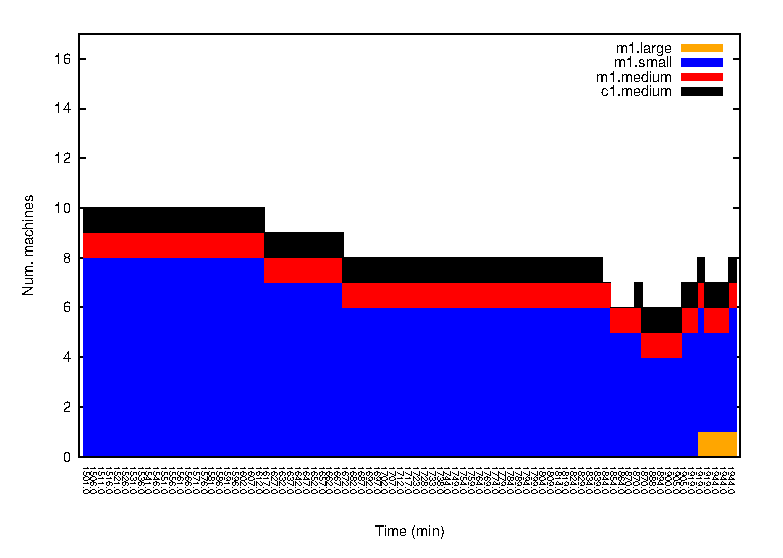
\includegraphics[height=4cm]{images/exps2011/medium/ec2/inst_type_machines_filtered.eps}
		\vspace{-4mm}
	\end{minipage}
\hfill
\begin{minipage}[b]{0.32\linewidth}
		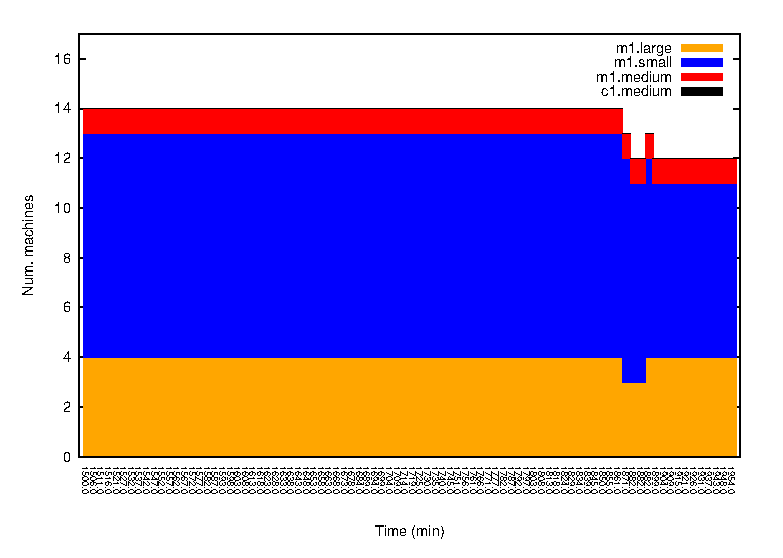
\includegraphics[height=4cm]{images/exps2011/high/ec2/inst_type_machines_filtered.eps}
		\vspace{-4mm}
	\end{minipage}
\caption{Cloud instances provisioned to handle the outage.}
\label{fig:EC2Instances}
\end{figure*}

\paragraph{SLO violation cost VS Infrastructure cost}

\begin{figure*}[htb]
	\begin{minipage}[b]{0.32\linewidth}
		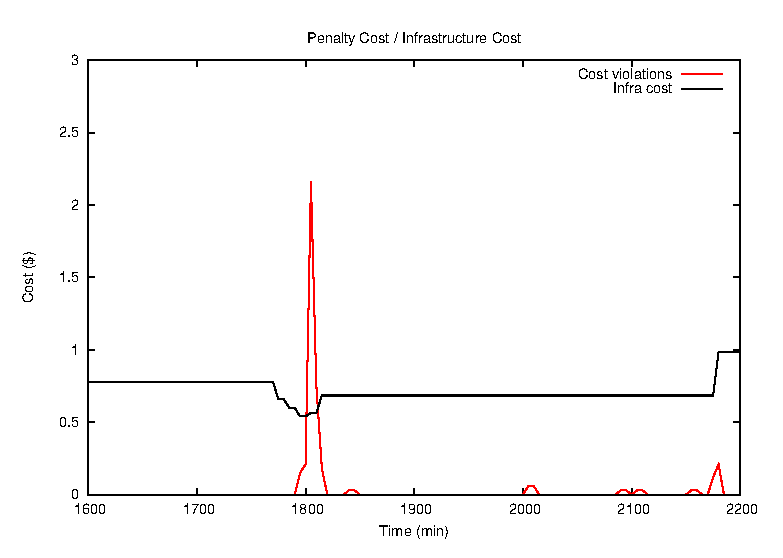
\includegraphics[height=4cm]{images/exps2011/low/ec2/penaltyVScost_filtered.eps}	
		\vspace{-4mm}
	\end{minipage}
	\hfill
	\begin{minipage}[b]{0.32\linewidth}
		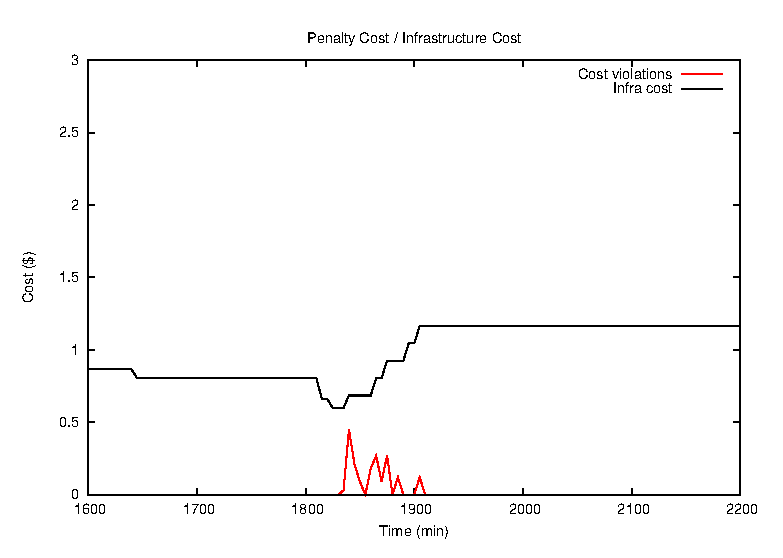
\includegraphics[height=4cm]{images/exps2011/medium/ec2/penaltyVScost_filtered.eps}
		\vspace{-4mm}
	\end{minipage}
\hfill
\begin{minipage}[b]{0.32\linewidth}
		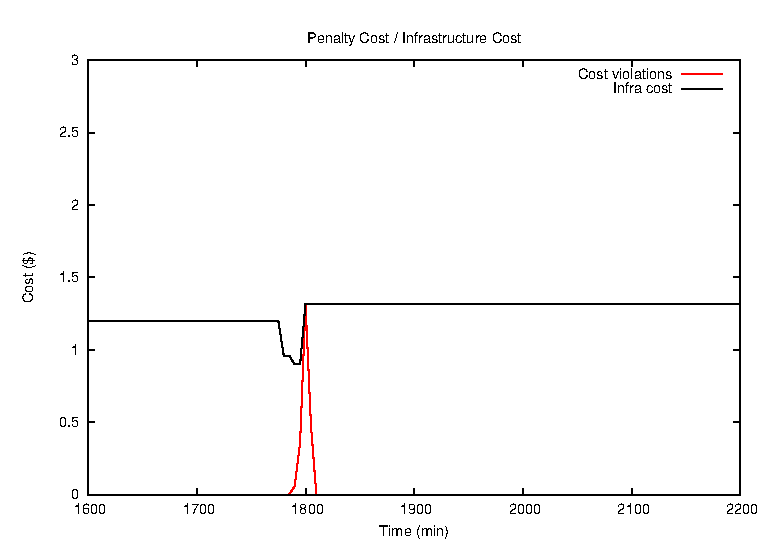
\includegraphics[height=4cm]{images/exps2011/high/ec2/penaltyVScost_filtered.eps}
		\vspace{-4mm}
	\end{minipage}
\caption{Cloud instances provisioned to handle the outage.}
\label{fig:EC2Penalty}
\end{figure*}


\begin{table*}\label{summaryEC2}
  {\scriptsize 
\begin{center}
    \begin{tabular}{  | c | c | c | c | c |}
    \hline
         \textbf{Name}  & \textbf{SLO Violations} & \textbf{Decisions}  & \textbf{Cost}  & \textbf{Cost violations} \\ \hline
   \textit{Bronze}   &  117 &  23 &  38.275 \$ &  \$ \\ \hline   
   \textit{Silver}  &  74 &  27 &  47,555 \$ &   \$ \\ \hline   
\textit{Gold} &   63  &  4 &  59.4 \$ &  \$ \\ \hline   

 \end{tabular}
\end{center}
\vspace{-5mm}
\caption{Analysis of results on EC2}
\label{summaryEC2}
}
\end{table*}


\subsubsection{Analysis of results}

%%% EXPERIMENTS DAS4 %%%%


\subsection{Homogeneous Infrastructure}

Our experiments on DAS-4 rely on OpenNebula as IaaS~\cite{sotomayor_virtual_2009}. To deploy the Wikipedia services, we initially provisioned small instances for the PHP service and one large instance for the MySQL service. Table~\ref{DAS4instances} detailed the hardware configurations of the different vm sizes in DAS-4.

\begin{table}\label{DAS4instances}
  {\scriptsize 
\begin{center}
    \begin{tabular}{  | c | c | c | c | }
    \hline
       \textbf{Name}  & \textbf{Configuration} & \textbf{Cost/hr} \\ \hline
   \textit{small}   & 1-core 2.4Ghz -- 1Gb RAM&  0.05\$ \\ \hline
   \textit{medium}   & 4-core 2.4Ghz  -- 4Gb RAM&  0.23\$ \\ \hline
\textit{highcpu-medium} & 6-core 2.4Ghz -- 3Gb RAM& 0.28\$   \\ \hline
\textit{large} & 8-core 2.4Ghz  -- 8Gb RAM& 0.46\$   \\ \hline

 \end{tabular}
\end{center}
\vspace{-5mm}
\caption{DAS4 instance type characteristics.}
\label{DAS4instances}
}
\end{table}


\paragraph{SLA fulfillment}


\begin{figure*}[htb]
	\begin{minipage}[b]{0.32\linewidth}
		\includegraphics[height=4cm]{images/exps2011/low/das/proxyDataPoints_output.eps}	
		\vspace{-4mm}
	\end{minipage}
	\hfill
	\begin{minipage}[b]{0.32\linewidth}
		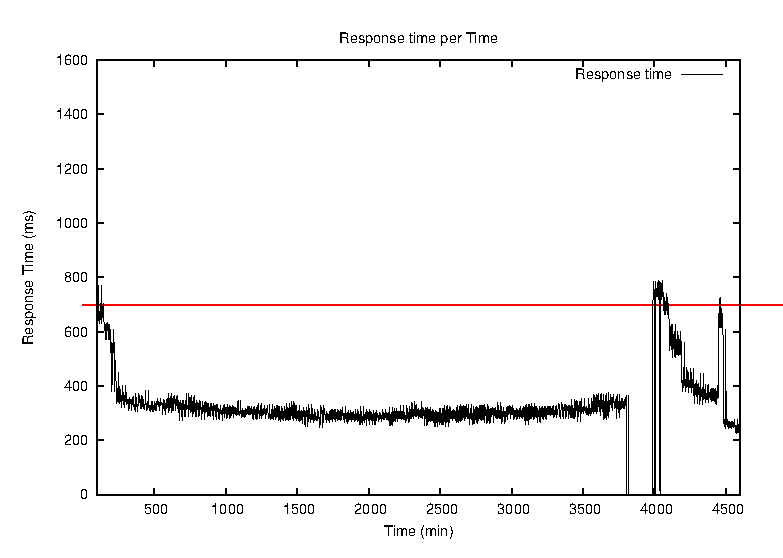
\includegraphics[height=4cm]{images/exps2011/medium/das/proxyDataPoints_output.eps}
		\vspace{-4mm}
	\end{minipage}
\hfill
\begin{minipage}[b]{0.32\linewidth}
		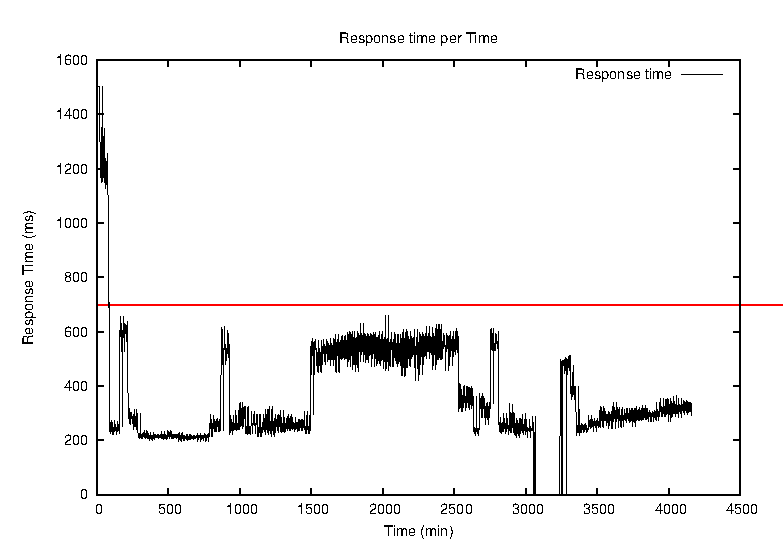
\includegraphics[height=4cm]{images/exps2011/high/das/proxyDataPoints_output.eps}
		\vspace{-4mm}
	\end{minipage}
\caption{Response time values during the outage.}
\label{fig:EC2ResponseTime}
\end{figure*}


\paragraph{Resource consumption}

\begin{figure*}[htb]
	\begin{minipage}[b]{0.32\linewidth}
		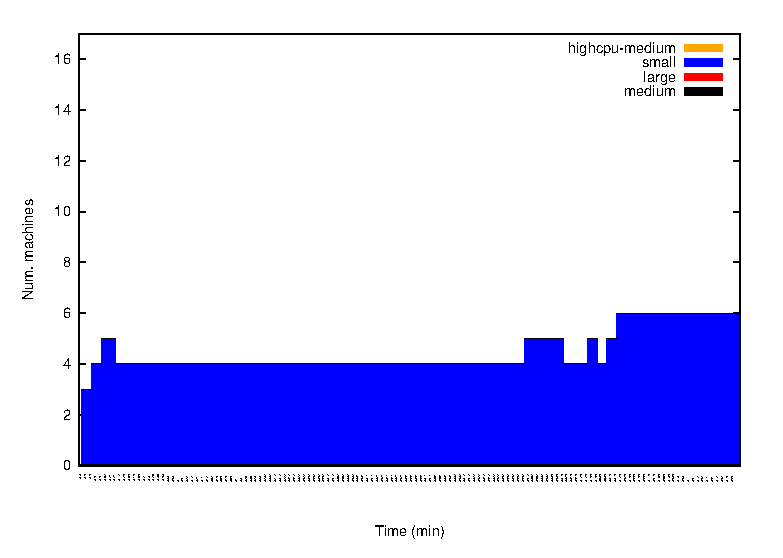
\includegraphics[height=4cm]{images/exps2011/low/das/inst_type_machines.eps}	
		\vspace{-4mm}
	\end{minipage}
	\hfill
	\begin{minipage}[b]{0.32\linewidth}
		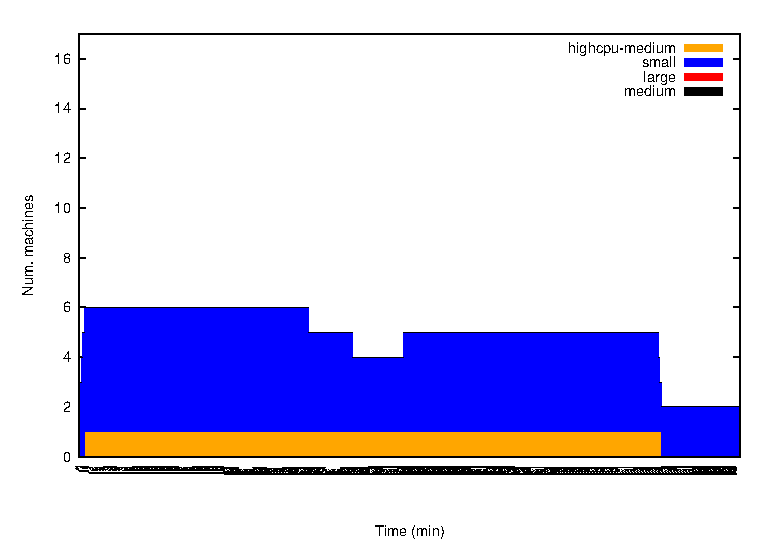
\includegraphics[height=4cm]{images/exps2011/medium/das/inst_type_machines.eps}
		\vspace{-4mm}
	\end{minipage}
\hfill
\begin{minipage}[b]{0.32\linewidth}
		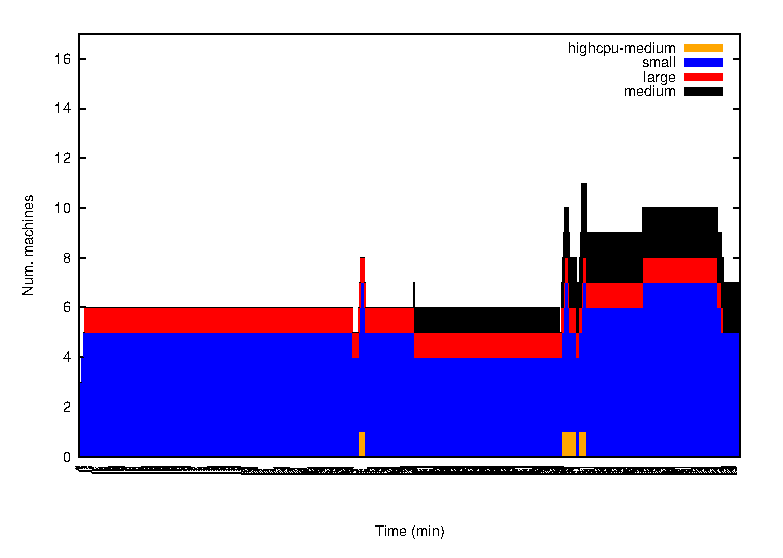
\includegraphics[height=4cm]{images/exps2011/high/das/inst_type_machines.eps}
		\vspace{-4mm}
	\end{minipage}
\caption{Cloud instances provisioned to handle the outage.}
\label{fig:DASInstances}
\end{figure*}

\paragraph{SLO violation cost VS Infrastructure cost}

\begin{figure*}[htb]
	\begin{minipage}[b]{0.32\linewidth}
		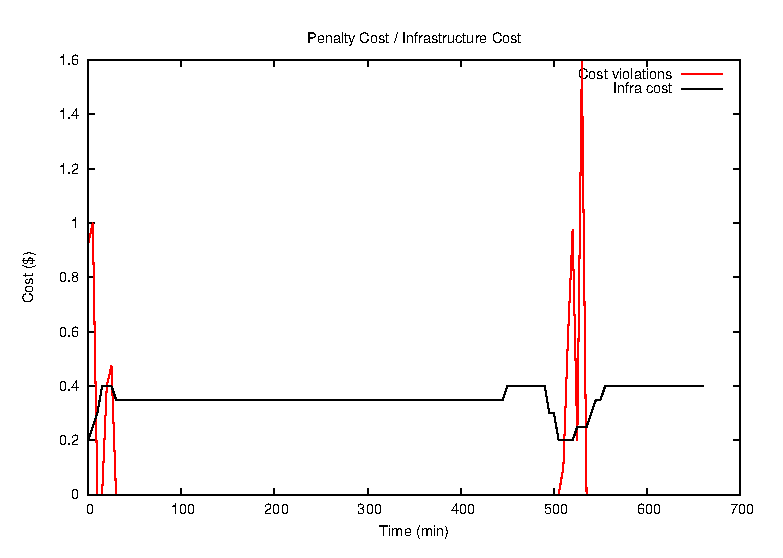
\includegraphics[height=4cm]{images/exps2011/low/das/penaltyVScost.eps}	
		\vspace{-4mm}
	\end{minipage}
	\hfill
	\begin{minipage}[b]{0.32\linewidth}
		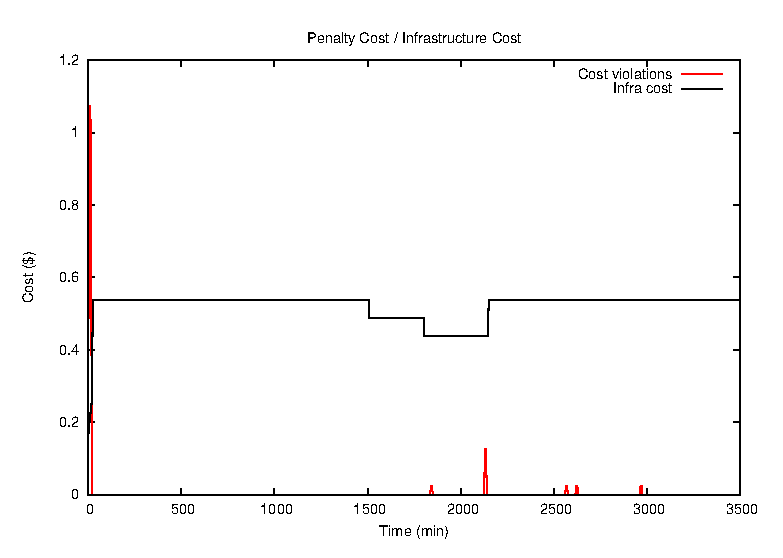
\includegraphics[height=4cm]{images/exps2011/medium/das/penaltyVScost.eps}
		\vspace{-4mm}
	\end{minipage}
\hfill
\begin{minipage}[b]{0.32\linewidth}
		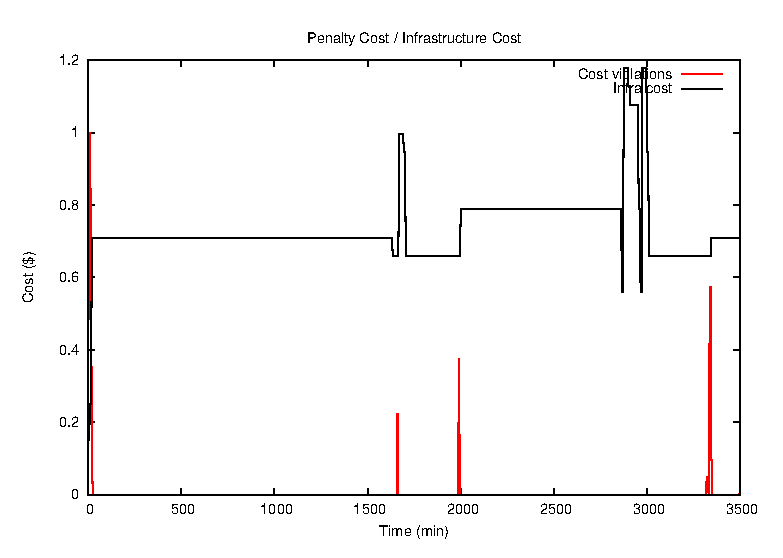
\includegraphics[height=4cm]{images/exps2011/high/das/penaltyVScost.eps}
		\vspace{-4mm}
	\end{minipage}
\caption{Cloud instances provisioned to handle the outage.}
\label{fig:DASPenalty}
\end{figure*}

\begin{table*}
  {\scriptsize 
\begin{center}
    \begin{tabular}{  | c | c | c | c | c |}
    \hline
         \textbf{Name}  & \textbf{SLO Violations} & \textbf{Decisions}  & \textbf{Cost}  & \textbf{Cost violations} \\ \hline
   \textit{A}   & 250  &  8 &  6.4 \$ &  \$ \\ \hline   
   \textit{B}  &   &   &   \$ &  4.5 \$ \\ \hline   
   \textit{C}  &  127 &  9 &  6.9 \$ &   \$ \\ \hline   
   \textit{D}  &   &   &   \$ &   \$ \\ \hline   
\textit{E} &  83 & 31 & 12.8 \$ &  \$ \\ \hline   

 \end{tabular}
\end{center}
\vspace{-5mm}
\caption{Analysis of results on DAS4}
\label{summaryDAS4}
}
\end{table*}

\subsubsection{Analysis of results}
